                 %\documentclass[a4paper,10pt]{article}
\documentclass[10pt]{article}
\usepackage[utf8]{inputenc}
\usepackage{xspace}
\usepackage{url}
\usepackage{graphicx,graphics} 
\usepackage{color}
\usepackage{caption}
\usepackage{amsmath}
\usepackage{amsfonts}
\usepackage{amssymb}
\usepackage{amsthm}
\usepackage{algorithm}
\usepackage{algorithmic}
\usepackage{longtable}
\usepackage{complexity}
\usepackage{tkz-graph}
\usepackage{float}
\usepackage{tabularx}
\usepackage{setspace}
\usepackage{icomma}
\renewcommand{\algorithmicrequire}{\textbf{Input:}}
\renewcommand{\algorithmicensure}{\textbf{Output:}}
\usepackage{authblk}
\usepackage[colorlinks=true,breaklinks=true,linkcolor=blue]{hyperref}


\newcommand\rmatching{${\cal R}$-matching\xspace}
\newcommand\mdelay{$\cal M$-delay\xspace}
\newcommand\matchedgraph{{\bf matched graph}}
\newtheorem{proposition}{Proposition}
\newtheorem{theorem}{Theorem}

\setlength{\parskip}{1ex} % Espace entre les paragraphes

\newtheorem{fact}{Fact}
\newtheorem{lemma}[theorem]{Lemma}
\newtheorem{definition}{Definition}
\newtheorem{corollary}{Corollary}

% \renewcommand{\thefootnote}{\*}

\newcommand{\todo}[1]{{\color{red} TODO: {#1}}}
\newcommand\pazl{\textsc{pazl}\xspace}
\newcommand\pall{\textsc{pall}\xspace}
\newcommand\bra{\textsc{bra}\xspace}
\newcommand\pra{\textsc{pra}\xspace}
\newcommand\minpra{\textsc{min-pra}\xspace}
%opening
\title{Deterministic Scheduling of Periodic Messages for Cloud RAN}
 

\author[1]{Dominique Barth}
\author[1,2]{Ma\"el Guiraud}
% \author[1]{Christian Cad\'er\'e}
 \author[2]{Brice Leclerc}
 \author[2]{Olivier Marc\'e}
\author[1]{Yann Strozecki}
\affil[1]{David Laboratory, UVSQ}
\affil[2]{Nokia Bell Labs France}

\begin{document}

\begin{section}{Topology, generation and problem}
\begin{subsection}{Model of the generated graphs}


The star topology has a conflict depth one. We now look at the topologies with a conflict depth two.
  
In order to generate some random digraphs $G=(V,A)$ of conflict depth two, we first generate some random bipartite graphs $G'=(V',E')$, which represent the core of the network. Indeed, it seems to be a good idea to model the internet topology as mentioned in \cite{tarissan_towards_2013}. This papers also gives us some background to generate some good random bipartite graphs. 
$V'$ is composed of two sets: The first set $S_1$, of size $a$, models the last switch before the data-centers, and the second set $S_2$, of size $b$, models some distant switches, reparted on the filed. We fix $a$ and $b$ and we uniformly draw the edges of $E'$ with a given probability. Note that $|E'|= a \times b$. If the generated graph  $G'$ is not connected, we generate another bipartite graph.
Figure~\ref{fig:random23} is an example of a random bipartite graph generated, with $a = 2$, $b=3$ and $|E'|=4$.

\begin{figure}[h]
\begin{center}
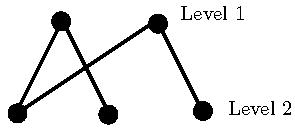
\includegraphics[width=0.5\textwidth]{random23}
\caption{A random bipartite graph $G'$.}\label{fig:random23}
\end{center}
\end{figure}


We now use $G'$ to build our routed network $G$
In order to create some arcs with conflict, the vertices of $G'$ are extended to become some arcs in $G$. Let us call \textbf{conflict arcs} those arcs. The egdes of $E'$ becomes some arcs of $A$, that we will call \textbf{core arcs}.

Figure~\ref{fig:extendnode} and figure~\ref{fig:extendendgraph} show how the first part of $G$ is build from $G'$.

\begin{minipage}{.5\linewidth}

\begin{center}
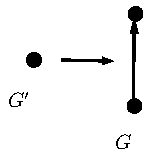
\includegraphics[width=0.4\textwidth]{extendnode}
\captionof{figure}{A node of $G'$ represent an arc in $G$.}\label{fig:extendnode}
\end{center}

\end{minipage}
\begin{minipage}{.5\linewidth}

\begin{center}
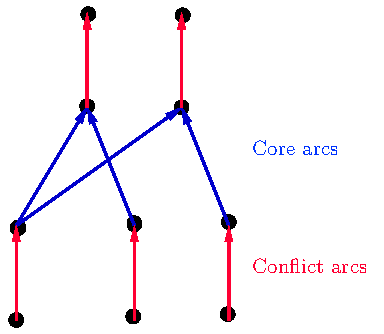
\includegraphics[width=0.4\textwidth]{extendendgraph}
\captionof{figure}{A node of $G'$ represent an arc in $G$.}\label{fig:extendendgraph}
\end{center}

\end{minipage}

 We now want to create some \textbf{final arcs}, that will model the last link before the antennas.
We generate $1\leq k\leq K$ final arcs before each contention arc $(u,v)$. We add $k$ new vertices $\{w_1,\ldots,w_k\}$ of indegree $0$ and outdegree $1$ to the set of vertices $V$. The new arcs $\{(w_1,u),\ldots,(w_k,u)\}$ are then added to $A$. 

Each route of the set of routes $\cal{R}$ of the routed network (G,$\cal{R}$) is composed either of one final arc and one contention arc (obtained from the set $S_1$ of arcs in $G'$), or one final arc, two contention arcs (one from $S_1$, one frome $S_2)$) and the core arc between those two contention arcs.
Note that one final arc belongs to one and only one route, while the core and contention arcs can be shared by several routes.

Figure~\ref{fig:extendendgraph2} and figure~\ref{fig:extendendgraph3} shows how the final arcs are generated and define the routes of the routed network (G,$\cal{R}$). The routes of the same color share the same arcs after the final arc.

\begin{minipage}{.5\linewidth}

\begin{center}
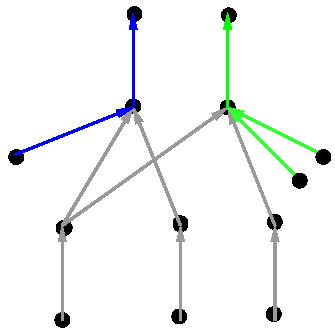
\includegraphics[width=0.4\linewidth]{extendendgraph2}
\captionof{figure}{Final arcs before contention arcs obtained from $S_1$.}\label{fig:extendendgraph2}
\end{center}

\end{minipage}
\begin{minipage}{.5\linewidth}
\begin{center}
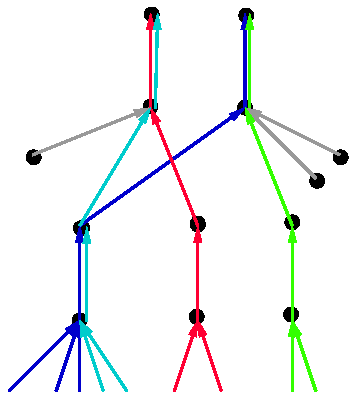
\includegraphics[width=0.4\linewidth]{extendendgraph3}
\captionof{figure}{Final arcs before contention arcs obtained from $S_2$.}\label{fig:extendendgraph3}
\end{center}
\end{minipage}
  The obtained routed network (G,$\cal{R}$) models a meshed network. The vertices of indegree $0$ of final arcs represent the antennas, the contention arcs from $S_1$ represent the last link before the datacenters, and the other nodes and arcs of the graph represent some links and switch of the network. It appears that this topology is realitic in core networks.
  Figure~\ref{fig:extendendgraphgrey} shows the shape of the network modelized.

\begin{figure}[h]
\begin{center}
 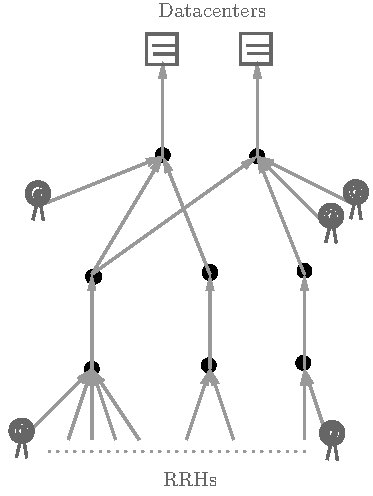
\includegraphics[width=0.4\textwidth]{extendendgraphgrey}
\caption{A network represented by a graph $G$.}\label{fig:extendendgraphgrey}
\end{center}
\end{figure}



  
  \end{subsection}
  
  \begin{subsection}{Different implemented algorithms}
  Consider that the size $\tau$ of the messages is the same for all routes. Also, the messages are sent in one packet, which can not be fragmented in the network.
  
  We first introduce a basic routine that helps us to test if the messages sent on a route at a given departure time can pass through the entire route without collisions.
  
    	\begin{algorithm}[H]
 	\caption{MessageCollisions}
 	\begin{algorithmic}
 	\REQUIRE A route $r$, a departure time, and a way of the message (FORWARD/BACKWARD).
	\ENSURE 1 if the messages can use the route with the given departure time, $0$ otherwise.

 	\FORALL{Arcs in the route}
 	\IF{ There is a collision with the previous scheduled messages}
 	\STATE return $0$
 	\ENDIF
 	\ENDFOR
	\STATE return $1$
 	\end{algorithmic}
 	\end{algorithm}
  \begin{subsection}{Algorithms without waiting times}
  \begin{subsubsection}{Greedy Prime}
  The idea here is to send the messages as soon as possible on each route. This is a greedy algorithm that does not try to optimize anything.

   	\begin{algorithm}[H]
 	\caption{Greedy Prime}
 	\begin{algorithmic}
 	\REQUIRE A graph, a set of routes, a period $P$
	\ENSURE A P-periodic assignment in p $\leq P$, or FAILURE

 	\FORALL{routes $i$ }
	\STATE tmp = $0$
	
 	\WHILE{!MessageCollisions($i$,tmp,FORWARD) $||$ !MessageCollisions($i$,tmp+routeLength($i$),BACKWARD) }
 	
 	\STATE tmp++;
 	\IF{tmp$ > P$}
	\STATE return FAILURE
	\ENDIF
 	\ENDWHILE
	\STATE DepartureTime($i$) = tmp;
 	\ENDFOR
	\STATE return departureTime
 	\end{algorithmic}
 	\end{algorithm}
	This algorithm treats the routes one by one by id (arbitrarily chosen), and set the departure time of the messages on the route as soon as possible.
  \end{subsubsection}
    \begin{subsubsection}{Greedy Min}
  
  We now try a smarter greedy algorithm. We start for the greedy algorithm proposed in \cite{Guir1806:Deterministic}.
  This algorithm works on one forward and one backward period. The idea is to cut the forward period in meta intervals of size $\tau$. Then, for each routes, we try each free meta interval in the forward period until the message can pass in the backward period without collisions. Here, the principle is the same, but instead of looking at only one backward period, we take into consideration all the contention points of the route in the same time. Since we did not study this topology enough for now, we do not have the theoretical result that ensure us to find a solution under a given load, but we use the idea of the algorithm and try to adapt it in order to optimize the chances of success. Indeed, instead of trying the meta intervals one by one and scheduling the route on the first meta interval that gives not collisions, we try to minimize the size lost in all the collisions points of the route.
 	The size lost is the number of tics between the end of the previous message and the beginning of the message scheduled.
	The goal is then to choose, for a route $i$ the meta interval that allow the message to pass though all the arc of its route without collisions, but also that minimise the sum of the size lost in every contention point of the route.
	
    	\begin{algorithm}[H]
 	\caption{sizeLost}
 	\begin{algorithmic}
 	\REQUIRE A route $r$, a departure time $t$
	\ENSURE $-1$ if the message can not pass without collisions, the size lost otherwise
	\STATE tmp  $\leftarrow$ $0$
 	\FORALL{Arcs $j$ in the route (forward AND backward)}
 	\IF{ There is a collision with the previous scheduled messages}
 	\STATE return $-1$
	\ELSE
	\STATE tmp += numberOfTicsLost(t,j)
 	\ENDIF
 	\ENDFOR
	\STATE return tmp
 	\end{algorithmic}
 	\end{algorithm}

	
   	\begin{algorithm}[H]
 	\caption{Greedy Min}
 	\begin{algorithmic}
 	\REQUIRE A graph, a set of routes, a period $P$
	\ENSURE A P-periodic assignment in p $\leq P$, or FAILURE

 	\FORALL{routes $i$ }
	\STATE minTicLost $\leftarrow$ INT MAX
	\STATE minId = $-1$
	\FORALL{ meta interval $j$ }
	\STATE tmp = sizeLost($r$,$j\times\tau$)
	\IF{ (tmp != $-1$)  AND (tmp < minTicLost)}
	\STATE minTicLost  $\leftarrow$ tmp
	\STATE minId  $\leftarrow$ $j$
	\ENDIF
 	\ENDFOR
	\IF{minId = $-1$}
	\STATE return FAILURE
	\ENDIF
	\STATE departureTime($i$) = $j\time\tau$
 	\ENDFOR
	\STATE return departureTime

 	\end{algorithmic}
 	\end{algorithm}

  \end{subsubsection}
  \end{subsection}
    \begin{subsection}{Algorithms with waiting times}
     We now allow the messages to be buffered in the BBUs. Thus we can manage the messages in both the RRH and the BBU.
    \begin{subsubsection}{Greedy Loaded}

In this algorithm, we choose to first take care of the more critical contention points first. Thus, we sort the arcs of the graph for the one in which there is the most of routes, to the one in which there is the less of routes. Then we take first the more loaded link and we schedule the routes on it in two steps.
First, we search the lowest departure time such that there is no collisions in the way forward, then we do it again on the way backward. Then, we can have some waiting times but it gives us a greater degrees of freedom to find an assignment.

   	\begin{algorithm}[H]
 	\caption{Greedy Loaded}
 	\begin{algorithmic}
 	\REQUIRE A graph, a set of routes, a period $P$
	\ENSURE A P-periodic assignment

 	\FORALL{arcs $i$ sorted by decreasing number of routes using $i$}
	
 	\FORALL{ route $j$ on $i$}
	\IF{$j$ has not been scheduled yet}
	\STATE tmp = $0$
	
 	\WHILE{!MessageCollisions($j$,tmp,FORWARD) }
 	
 	\STATE tmp++;
 	\IF{tmp$ > P$}
	\STATE return FAILURE
	\ENDIF
 	\ENDWHILE
	\STATE DepartureTime($j$) = tmp;
	\STATE tmp2 = tmp + routeLength($j$);
	\STATE tmp = tmp2;
	
 	\WHILE{!MessageCollisions($j$,tmp,BACKWARD) }
 	
 	\STATE tmp++;
 	\IF{tmp$ > P+tmp2$}
	\STATE return FAILURE
	\ENDIF
 	\ENDWHILE
	\STATE waitingTime($j$) = tmp-tmp2;
	\ENDIF
 	\ENDFOR

 	\ENDFOR
	\STATE return departureTime, waitingTime

 	\end{algorithmic}
 	\end{algorithm}

    \end{subsubsection}
  \end{subsection}
\end{subsection}
\end{section}
\bibliographystyle{ieeetr}
\bibliography{srcs}
\end{document}
